\section{Case Study: Verification of \texttt{[T]::binary\_search}}
\label{sec:binary_search}

As a first test of the translation tool, we set out to verify the correctness
of the binary search implementation in the Rust standard library, an algorithm of
medium complexity.

\subsection{The Rust Implementation}

Before we can even tackle the algorithmic complexity, we have to cope with the
design complexity of a real-world library. The public implementation of the
\rust{binary_search} method implemented on any slice type can be found in the \rust{collections} crate.

\begin{minted}{rust}
use core::slice as core_slice;

impl<T> [T] {
  ...

  /// Binary search a sorted slice for a given element.
  ///
  /// If the value is found then `Ok` is returned, containing the
  /// index of the matching element; if the value is not found then
  /// `Err` is returned, containing the index where a matching
  /// element could be inserted while maintaining sorted order.
  ///
  /// ...
  pub fn binary_search(&self, x: &T) -> Result<usize, usize>
    where T: Ord {
    core_slice::SliceExt::binary_search(self, x)
  }
}
\end{minted}

As we can see from the its documentation and signature, the method
is very general: It works on all slices whose element type implements the
\rust{Ord} trait, and it returns information in both the success and the failure
case. The implementation, however, turns out to be merely a redirection to a
trait method in the base crate \rust{core}. This trait has a single
implementation, for the slice type.

\begin{minted}{rust}
pub trait SliceExt {
  type Item;

  fn binary_search(&self, x: &Item) -> Result<usize, usize>
    where Item: Ord;
  fn len(&self) -> usize;
  fn is_empty(&self) -> bool { self.len() == 0 }
  ...
}

impl<T> SliceExt for [T] {
  type Item = T;

  fn binary_search(&self, x: &T) -> Result<usize, usize> where T: Ord {
    self.binary_search_by(|p| p.cmp(x))
  }
  fn len(&self) -> usize { ... }
  ...

}
\end{minted}

This indirection seems pointless at first, but follows from a technical
restriction: There may be at most one \rust{impl} block for a primitive type
like \rust{[T]}. Because the \rust{core} crate does not depend on the existence
of a heap allocator, but some methods on \rust{[T]} like its merge sort
implementation do need dynamic allocation, the \rust{impl} block is only
declared in the later \rust{collections} crate. Since \rust{binary_search} does
not need an allocator, it should still reside in \rust{core}, and instead is
associated to the slice type via the helper trait.

\begin{listing}[!bt]
\begin{minted}{rust}
fn binary_search_by<'a, F>(&'a self, mut f: F) -> Result<usize, usize>
    where F: FnMut(&'a T) -> Ordering
{
    let mut base = 0usize;
    let mut s = self;

    loop {
        let (head, tail) = s.split_at(s.len() >> 1);
        if tail.is_empty() {
            return Err(base)
        }
        match f(&tail[0]) {
            Less => {
                base += head.len() + 1;
                s = &tail[1..];
            }
            Greater => s = head,
            Equal => return Ok(base + head.len()),
        }
    }
}
\end{minted}
  
\caption{Implementation of the \rust{binary_search_by} method. A subslice
  \rust{s} of \rust{self} is iteratively bisected until it is empty or the
  element has been found. The \rust{tail[1..]} \emph{slicing syntax} is
  syntax sugar for \rust{tail.index(RangeFrom{start: 1})}.}
\label{lst:binary_search_by}
\end{listing}

This final version of \rust{binary_search}, which we represent as
\rust{core::<[T] as SliceExt>::binary_search}, is implemented by way of a more
general method \rust{binary_search_by} that takes a comparison function instead
of being constrained to \rust{Ord} (\autoref{lst:binary_search_by}). This
method, finally, turns out to be much more abstract than one might expect: Instead of
the standard binary search implementation that iteratively reduces the search range via two
indices, the range is represented as a subslice and manipulated via high-level
slice methods such as \rust{split_at}. The reasoning behind this is a great show
case for Rust's zero-cost (or even negative-cost, in this case) abstractions
philosophy -- the abstract implementation actually surpasses a direct
implementation in terms of efficiency because it helps the compiler to eliminate
all bounds checks in it. It also elegantly avoids the common
pitfall\footnote{https://research.googleblog.com/2006/06/extra-extra-read-all-about-it-nearly.html}
of a potential integer overflow in less abstract code like \rust{mid = (low + high) / 2}.

\newgeometry{bottom=1cm}
\begin{sidewaysfigure}
  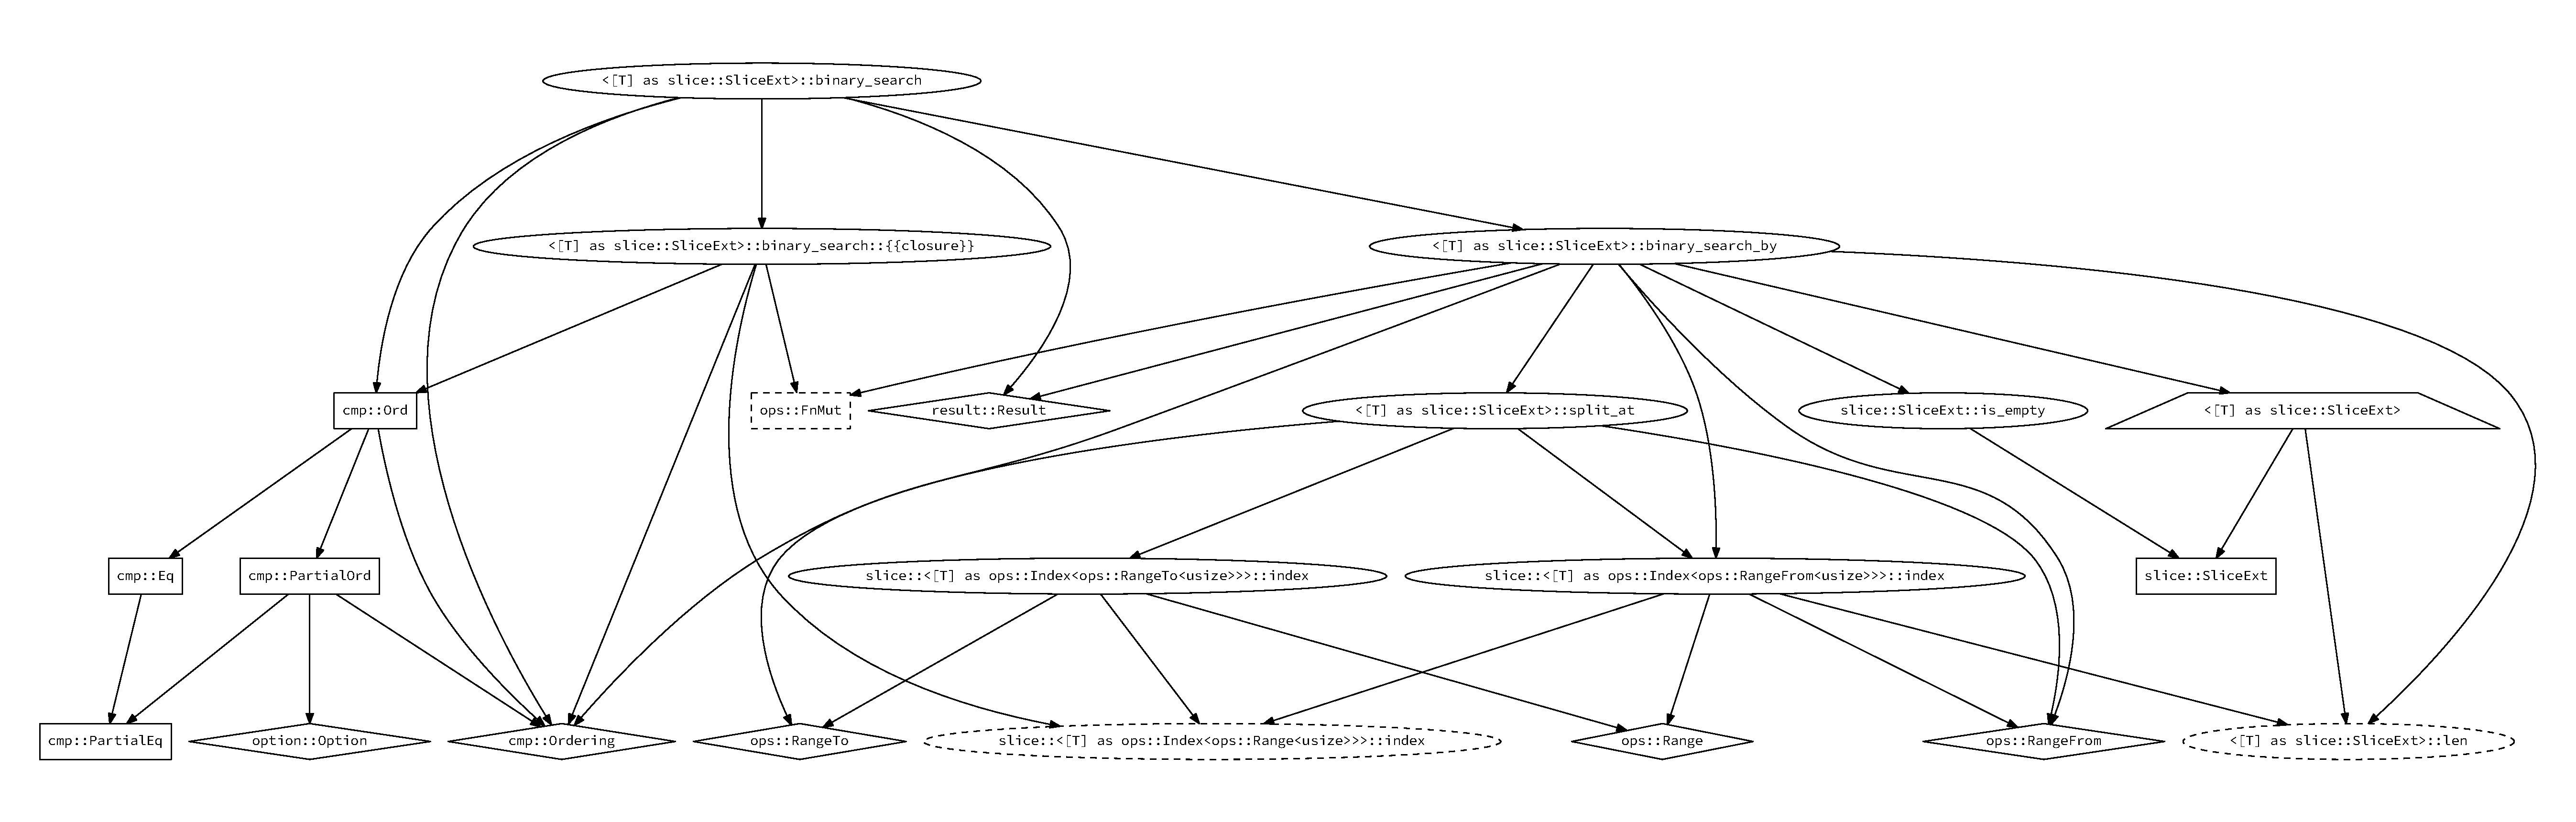
\includegraphics[width=\textheight]{deps}
  \caption[A complete graph of the dependencies of \rust{binary_search}]{A
    complete graph of the translation dependencies of \rust{binary_search} in
    the \rust{core} crate,
    distinguishing between \tikz[baseline=-0.3em]\node[draw, shape=ellipse] {functions};,
    \tikz[baseline=-0.3em]\node[draw, shape=rectangle] {types};,
    \tikz[baseline=-0.3em]\node[draw, shape=diamond, aspect=2] {traits};,
    and \tikz[baseline=-0.3em]\node[draw, shape=trapezium] {trait
      implementations};. Axiomatized items that use unsafe code in the original
    implementation are marked by dashed borders. Because
    we eagerly resolve trait method calls where possible, such as to the
    \rust{index} method of \rust{Index<RangeFrom<usize>>} for \rust{[T]}, we can
    avoid some dependencies like the full \rust{Index} implementation for
    \rust{[T]}, and even the trait itself.
  }
  \label{fig:deps}
\end{sidewaysfigure}
\restoregeometry

For our purposes, the abstract implementation primarily means a fair number of
additional dependencies we have to support and inspect~(\autoref{fig:deps}). All
in all, \rust{binary_search} turned out to be an ideal first test not only because
of its algorithmic complexity, but also because of its use of numerous Rust
language features including enums, structs, traits with associated types and
default methods, higher-order functions, and loops.

\subsection{Prelude: Coping with Unsafe Dependencies}

When trying to translate the \rust{binary_search} method including its
dependencies, we will not get back a working definition at first. Our tool
refuses to translate some dependencies because they use unsafe code, as marked
in \autoref{fig:deps}. We will have to translate these functions manually,
basically adding the correctness of their translation as axioms to the project.

Apart from our custom translation of \rust{FnMut} we discussed in
\autoref{sec:lambda}, both axiomatized functions operate on slices and are straightforward to
implement using our identification of slices with Lean lists.

\begin{minted}{lean}
-- Returns the number of elements in the slice.
definition «[T] as core.slice.SliceExt».len {T : Type₁} (self : slice T) : sem nat :=
return (list.length self)

-- Implements slicing with syntax `&self[begin .. end]`.
-- Returns a slice of self for the index range [`begin`..`end`).
-- This operation is `O(1)`.
-- Requires that `begin <= end` and `end <= self.len()`,
-- otherwise slicing will panic.
definition «[T] as core.ops.Index<core.ops.Range<usize>>».index {T : Type₁} (self : slice T) (index : Range usize) : sem (slice T) :=
sem.guard (Range.start index ≤ Range.«end» index ∧ Range.«end» index ≤ list.length self)
  (return (list.firstn (Range.«end» index - Range.start index) (list.dropn (Range.start index) self)))
\end{minted}

The latter method presents a
small technical hurdle: It is dependent on other translation products,
specifically the \lean{Range} structure. Instead of having to axiomatize that
perfectly translatable item and adding both definitions manually to the
\verb!pre.lean! file, we instruct the translator in the \verb!config.toml! file to inject our
Lean definition of \rust{index} as the translation of the Rust definition on-the-fly.

\begin{minted}{text}
[replace]
"«[T] as core.ops.Index<core.ops.Range<usize>>».index" = "..."
\end{minted}

\subsection{Formal Specification}

Going back to the original definition of \rust{[T]::binary_search}, we translate
the documented behavior into a Lean predicate.

\begin{minted}{lean}
parameters {T : Type₁} [Ord T]
parameter self : slice T
parameter needle : T -- a more descriptive name for the parameter `x`

inductive binary_search_res : Result usize usize → Prop :=
| found     : Πi, list.nth self i = some needle → binary_search_res (Result.Ok i)
| not_found : Πi, needle ∉ self → sorted (list.insert_at self i needle) →
  binary_search_res (Result.Err i)
\end{minted}

It is specifications like these where the power of shallow embeddings really
shines: We can freely mix and match Rust types and standard Lean functions and
constructs. In fact, we will have to do some more mixing of these two worlds to make
the definition valid: While we have copied the assumption \rust{T : Ord} from
the \rust{binary_search} method, the \lean{sorted} predicate expects T to
implement Lean's own ordering typeclass. We therefore introduce a new typeclass
\lean{Ord'} that merges both typeclasses -- or rather, in the Lean case, the
subclass of decidable, linear orders.

\begin{minted}{lean}
definition ordering {T : Type} [decidable_linear_order T] (x y : T) : cmp.Ordering :=
if x < y then Ordering.Less
else if x = y then Ordering.Equal
else Ordering.Greater

structure Ord' [class] (T : Type₁) extends Ord T, decidable_linear_order T :=
(cmp_eq : ∀ x y : T, Σ k, cmp x y = some (ordering x y, k))
\end{minted}

After changing the \lean{parameter} definition to \lean{Ord' T}, the
specification typechecks. We need two more (sensible) hypotheses before we can
prove that \lean{binary_search} upholds the specification.

\begin{minted}{lean}
hypothesis Hsorted : sorted self
hypothesis His_slice : is_slice self

...

theorem binary_search.spec : sem.terminates_with
  binary_search_res
  (binary_search self needle) := ...
\end{minted}

\subsection{Proof}

The full correctness proof is about 170 lines in Lean's tactic mode. We will not
discuss the individual steps or the Lean tactic syntax here, but focus on the main
proof steps.

After unfolding the \lean{binary_search} and \lean{binary_search_by}
definitions and some simplifications, we quickly reduce the proof obligation
down to the central loop.

\begin{minted}{lean}
⊢ sem.terminates_with binary_search_res
    (loop loop_4 (closure_5594.mk needle, 0, self))
\end{minted}

Here \lean{loop_4} is the loop body extracted from \lean{binary_search_by},
which is passed to the loop combinator \lean{loop} together with the initial
loop state. The loop state is the triple \lean{(f, base, s)} of local variables
mutated in the loop, initialized to the closure from \lean{binary_search}
(capturing \lean{needle}), \lean{0}, and \lean{self}, respectively. As described
in \autoref{sec:loop}, we can reduce the goal to one basing the loop on a
specific relation by use of the lemma \lean{loop.fix_eq_loop}.

\begin{minted}{lean}
abbreviation f₀ := closure_5594.mk needle
abbreviation loop_4.state := closure_5594 T × usize × slice T
definition R := measure (λ st : loop_4.state, length st.2)
...

⊢ sem.terminates_with binary_search_res
  (loop.fix loop_4 R (f₀, 0, self))
\end{minted}

\lean{measure} lets us create a well-founded relation on the loop state triple
by comparing the length of \lean{s}. We will not be able to show the new goal
directly via well-founded induction over \lean{R}, instead we first have to
generalize it. For that we first declare the loop invariants (which we obtained by
the non-sophisticated method of repeated try-and-error).

\begin{minted}{lean}
variables (base : usize) (s : slice T)

structure loop_4_invar :=
(s_in_self  : s ⊑ₚ (dropn base self))
(insert_pos : sorted.insert_pos self needle ∈ '[base, base + length s])
(needle_mem : needle ∈ self → needle ∈ s)
\end{minted}

These say that
\begin{enumerate}
\item \lean{s} is a contiguous subsequence of the original slice \lean{self} starting at \lean{base}; here \lean{⊑ₚ} is a
  notation for the (non-strict) list prefix order that will come in handy at multiple points
  in the proof.
\item inserting \lean{needle} at the first position in \lean{self} that will
  keep it sorted will insert it inside or adjacent to \lean{s}.
\item if \lean{needle} is at all in the original slice, it will also be in
  \lean{s}. If this is the case, this invariant will imply the previous one, but in
  general they are independent.
\end{enumerate}

Because the invariants trivially hold for the initial state, we can generalize
the goal.

\begin{minted}{lean}
⊢ loop_4_invar base s → sem.terminates_with binary_search_res
    (loop.fix loop_4 R (f₀, base, s))
\end{minted}

There is no need to generalize \rust{f₀} because we know it is a non-modifying closure
and thus the variable \rust{f} will always contain that value.

After applying well-founded recursion, we unroll one iteration of
\lean{loop.fix} via the lemma \lean{loop.fix_eq} from \autoref{sec:loop} and
apply the induction hypothesis on the loop remainder to reduce the goal to that
single iteration.

\begin{minted}{lean}
inductive loop_4_step : loop_4.state → Prop :=
mk : Π base' s', loop_4_invar base' s' → length s' ≤ length s / 2 → length s ≠ 0 →
  loop_4_step (f₀, base', s')


⊢ loop_4_invar base s → sem.terminates_with
    (sum.rec (loop_4_step s) binary_search_res)
    (loop_4 R (f₀, base, s))
\end{minted}

If the iteration breaks the loop (returns some \lean{sum.inr}), we need the
result to fulfill the top-level specification \lean{binary_search_res}.
Otherwise, if the loop produces
some new loop state \lean{(f₀, base', s')}, the loop invariants should be upheld
together with a loop \emph{variant} saying that the length of \lean{s} has at
least halved. Together with the information that \lean{length s ≠ 0}, this
implies \lean{length s' < length s} and ensures we can apply the induction
hypothesis. We will
need the former two stronger statements for proving the function's logarithmic
complexity below.

The remainder of the proof, while tedious, uses mostly basic reasoning. We split
the goal according to the \rust{if} and \rust{match} branches in the original
code and, depending on the return value in each case, show that
\lean{loop_4_invar} or \lean{binary_search_res} is upheld. We prove that neither
of the two additions in the code overflows by showing that they are bounded by
\lean{list.length self}, which by the assumption \lean{is_slice self} fits into
the \rust{usize} type.